\documentclass{article}
\usepackage{booktabs}
\usepackage{geometry}
\usepackage{graphicx}
\usepackage{setspace}
\usepackage{rotating}
\geometry{a4paper, margin=0.5in}
\begin{document}
\graphicspath{{BICPlots/}}


\begin{figure}[!ht]
Figure 1: BIC Plots. This figure shows the plots of Bayesian Information Criterion (BIC) value against moving average window size (m) for all the specifications of the MF2-GARCH-in-mean model \textit{(see Table 4 for parameter estimates)}. The optimal m value is chosen as the one that minimizes the BIC. The left column shows proportional variants and the right column shows the non-proportional ones. From top to bottom, the rows show the plots for the short-term component specification, the long-term component specification, the two component specification and the overall conditional variance specification.\\
\begin{center}
\begin{spacing}{0.5}
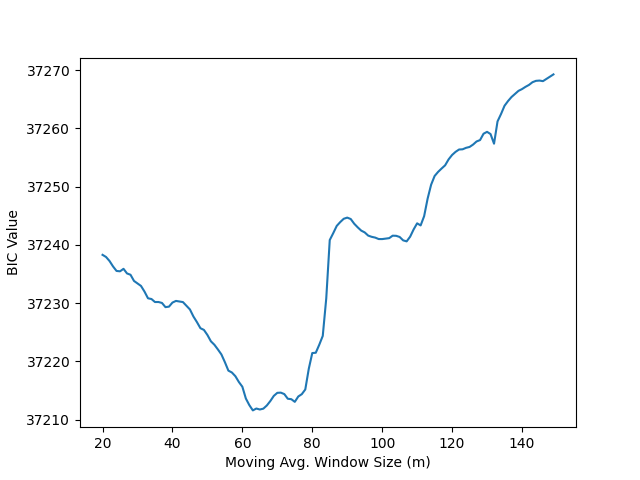
\includegraphics[scale=0.3]{Prop_ST_Cr}
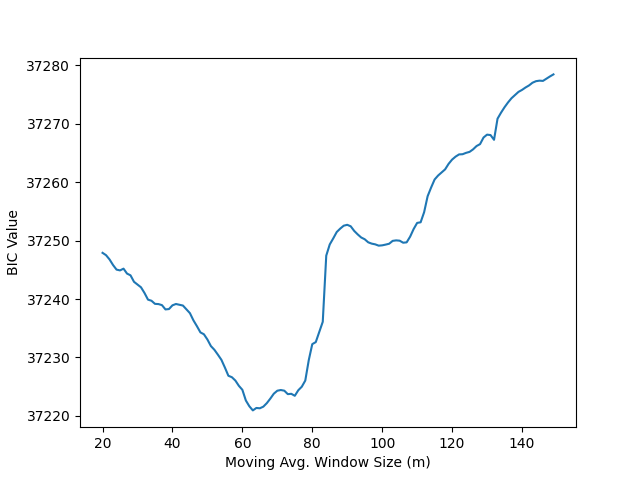
\includegraphics[scale=0.3]{ST_Cr}
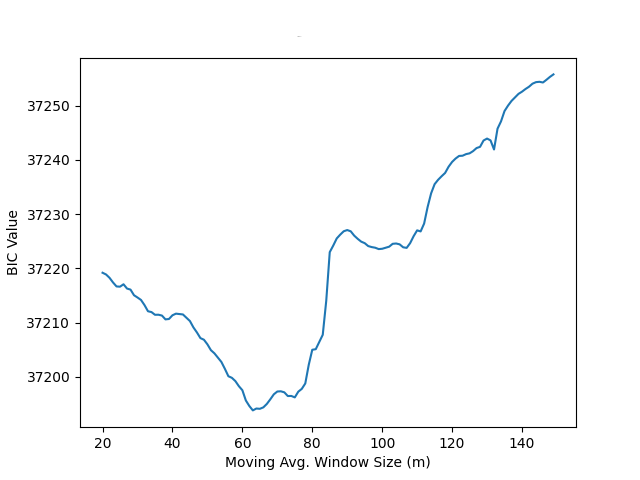
\includegraphics[scale=0.3]{Prop_LT_Cr}
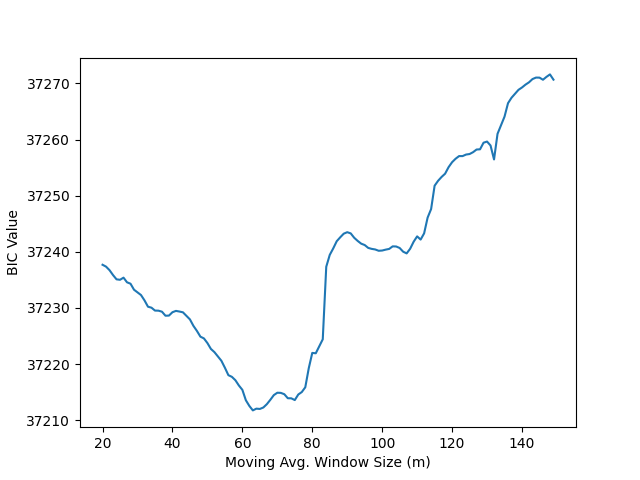
\includegraphics[scale=0.3]{LT_Cr}
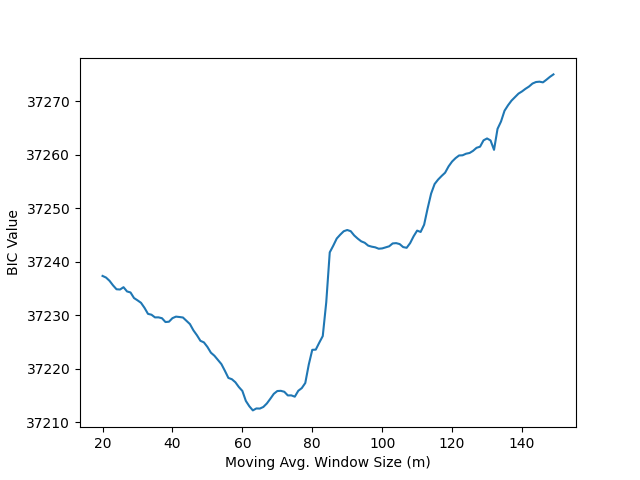
\includegraphics[scale=0.3]{Prop_Both_Cr}
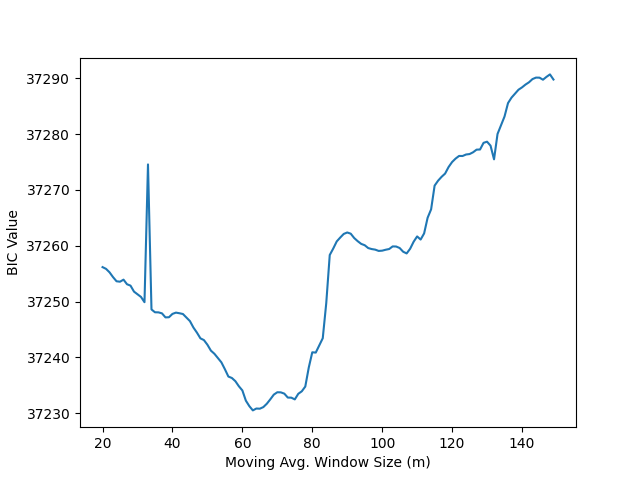
\includegraphics[scale=0.3]{Both_Cr}
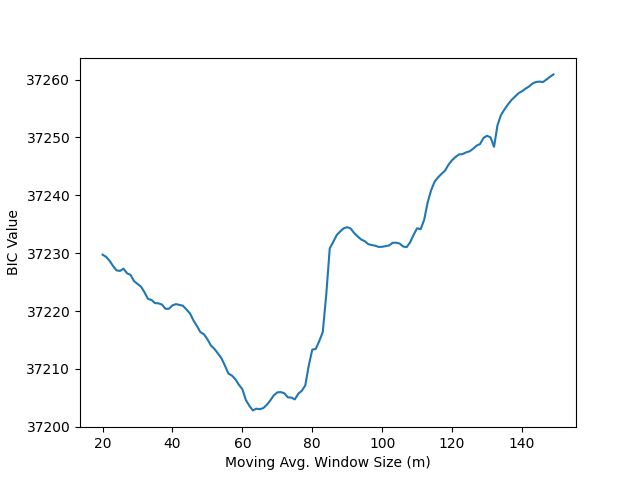
\includegraphics[scale=0.3]{Prop_Vol_Cr}
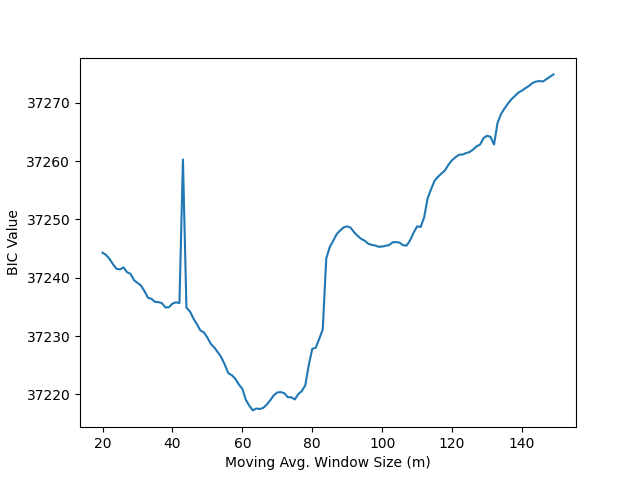
\includegraphics[scale=0.3]{Vol_Cr}
\end{spacing}
\end{center}
\end{figure}

\newpage
\begin{table}
\centering
\caption{Parameter Values for Monte Carlo Simulations}
\begin{tabular}{ccccccccccc}
\midrule
\midrule
$\alpha$ & $\gamma$ & $\beta$ & $\lambda_0$ & $\lambda_1$ & $\lambda_2$ & $\delta_0$ & $\delta_{1,s}$ & $\delta_{1,l}$ & $\delta_{1}$\\
\midrule
\multicolumn{11}{c}{\textbf{Short-term component}}\\
\multicolumn{11}{l}{Proportional}\\
0.006 & 0.160 & 0.842 & 0.011 & 0.085 & 0.902 & - & 0.027 & - & -\\
\multicolumn{11}{l}{Non-Proportional}\\
0.006 & 0.160 & 0.842 & 0.011 & 0.085 & 0.902 & 0.033 & -0.003 & - & -\\
\midrule
\multicolumn{11}{c}{\textbf{Long-term component}}\\
\multicolumn{11}{l}{Proportional}\\
0.006 & 0.160 & 0.842 & 0.011 & 0.085 & 0.902 & - & - & 0.049  & -\\
\multicolumn{11}{l}{Non-Proportional}\\
0.006 & 0.160 & 0.842 & 0.011 & 0.085 & 0.902 & 0.003 & - & 0.045 & -\\
\midrule
\multicolumn{11}{c}{\textbf{Both components (additive)}}\\
\multicolumn{11}{l}{Proportional}\\
0.006 & 0.160 & 0.842 & 0.011 & 0.085 & 0.902 & - & -0.005 & 0.054 & -\\
\multicolumn{11}{l}{Non-Proportional}\\
0.006 & 0.160 & 0.842 & 0.011 & 0.085 & 0.902 & 0.008 & -0.008 & 0.046 & -\\
\midrule
\multicolumn{11}{c}{\textbf{Overall conditional variance (multiplicative)}}\\
\multicolumn{11}{l}{Proportional}\\
0.006 & 0.160 & 0.842 & 0.011 & 0.085 & 0.902 & - & - & - & 0.042\\
\multicolumn{11}{l}{Non-Proportional}\\
0.006 & 0.160 & 0.842 & 0.011 & 0.085 & 0.902 & 0.020 & - & - & 0.023\\
\midrule
\multicolumn{11}{l}{\textbf{Notes:} This table presents the "true" parameter values I used in Monte Carlo}\\
\multicolumn{11}{l}{simulations of daily market premium data. The MF2-GARCH-in-mean model}\\
\multicolumn{11}{l}{is fitted $R=1,000$ times on these simulated samples, each of size $T=15,120$.}\\
\multicolumn{11}{l}{This is repeated for the proportional and non-proportional variant of every}\\
\multicolumn{11}{l}{specification. These values were chosen based on estimates from real data \textit{(see}}\\
\multicolumn{11}{l}{\textit{Table 4 below).}}\\
\midrule
\midrule
\end{tabular}
\end{table}

\pagebreak
\begin{table}[t]
\centering
\caption{Summary Statistics - Market Premia}
\begin{tabular}{cccccccc}
\midrule
\midrule
\mbox{} & mean & sd & skew & kurtosis & min & max & AC(1)\\
\midrule
$r_t$ & 0.028 & 1.028 & -0.487 & 15.564 & -17.440 & 11.360 & 0.016\\
\midrule
\multicolumn{8}{l}{\textbf{Notes:} This table shows summary statistics for the U.S. daily}\\
\multicolumn{8}{l}{market premium data. The data runs from January 1964 to April}\\
\multicolumn{8}{l}{2025. The columns present the mean, standard deviation (sd),}\\
\multicolumn{8}{l}{skewness, kurtosis, minimum (min), maximum (max) and the}\\
\multicolumn{8}{l}{first-order autocorrelation coefficient (AC(1)).}\\
\midrule
\midrule
\end{tabular}
\end{table}

\pagebreak
\begin{table}
\centering
\caption{NBER Recession Periods}
\begin{tabular}{ccl}
\midrule
\midrule
Start date & End date & Remarks\\
\midrule
December 1969 & November 1970 & - \\
November 1973 & March 1975 & 1973 oil crisis and stagflation \\
January 1980 & July 1980 & Volcker recession I \\
July 1981 & November 1982 & Volcker recession II \\
July 1990 & March 1991 & - \\
March 2001 & November 2001 & Dot-com bubble \\
December 2007 & June 2009 & Global financial crisis \\
February 2020 & April 2020 & COVID-19 pandemic \\
\midrule
\multicolumn{3}{l}{\textbf{Notes:} This table shows the start and end dates of recession}\\
\multicolumn{3}{l}{periods defined by the U.S. National Bureau of Economic}\\
\multicolumn{3}{l}{Research (NBER) which fall within the sample period on which}\\
\multicolumn{3}{l}{the MF2-GARCH-in-mean model is estimated. The dummy}\\
\multicolumn{3}{l}{variable used to control for periods of crisis is given the value 1}\\
\multicolumn{3}{l}{for the above periods and 0 otherwise.}\\
\midrule
\midrule
\end{tabular}
\end{table}

\newgeometry{a4paper, margin=0.2in}
\setcounter{table}{3}
\begin{sidewaystable}[t]
\centering
\caption{Combined Specification Parameter Estimates (Controlling for Crises)}
\begin{tabular}{ccccccccccccccccc}
\midrule
\midrule
$\alpha$ & $\gamma$ & $\beta$ & $\lambda_0$ & $\lambda_1$ & $\lambda_2$ & $\delta_0$ & $\delta_{1,s}$ & $\delta_{1,l}$ & $\delta_{1}$ & $\theta_0$ & $\theta_{1,s}$ & $\theta_{1,l}$ & $\theta_{1}$ & \mbox{LLF} & \mbox{BIC} \\

\midrule
\multicolumn{17}{c}{\textbf{Panel A: Short-term component}}\\
\multicolumn{17}{l}{Proportional}\\
\begin{tabular}[t]{@{}c@{}}0.007 \\ \small (0.014)\end{tabular}   & \begin{tabular}[t]{@{}c@{}}0.158*** \\ \small (0.019)\end{tabular}   & \begin{tabular}[t]{@{}c@{}}0.841*** \\ \small (0.018)\end{tabular}   & \begin{tabular}[t]{@{}c@{}}0.012 \\ \small (0.020)\end{tabular}   & \begin{tabular}[t]{@{}c@{}}0.086 \\ \small (0.150)\end{tabular}   & \begin{tabular}[t]{@{}c@{}}0.900*** \\ \small (0.173)\end{tabular}   & \mbox{-}   & \begin{tabular}[t]{@{}c@{}}0.027** \\ \small (0.011)\end{tabular}   & \mbox{-}   & \mbox{-}   &\mbox{-}   & \begin{tabular}[t]{@{}c@{}}-0.013 \\ \small (0.020)\end{tabular}   & \mbox{-}   & \mbox{-} & \mbox{-18567} &\mbox{37212}  \\
\multicolumn{17}{l}{Non-Proportional}\\
\begin{tabular}[t]{@{}c@{}}0.005* \\ \small (0.003)\end{tabular}   & \begin{tabular}[t]{@{}c@{}}0.166*** \\ \small (0.015)\end{tabular}   & \begin{tabular}[t]{@{}c@{}}0.845*** \\ \small (0.012)\end{tabular}   & \begin{tabular}[t]{@{}c@{}}0.011*** \\ \small (0.002)\end{tabular}   & \begin{tabular}[t]{@{}c@{}}0.081*** \\ \small (0.018)\end{tabular}   & \begin{tabular}[t]{@{}c@{}}0.907*** \\ \small (0.018)\end{tabular}   & \begin{tabular}[t]{@{}c@{}}0.033*** \\ \small (0.007)\end{tabular}   & \begin{tabular}[t]{@{}c@{}}-0.003*** \\ \small (0.001)\end{tabular}   & \mbox{-}   & \mbox{-}   & \begin{tabular}[t]{@{}c@{}}0.009\\ \small (0.008)\end{tabular} & \begin{tabular}[t]{@{}c@{}}-0.009 \\ \small (0.009)\end{tabular}   & \mbox{-}   & \mbox{-} & \mbox{-18562} &\mbox{37221}  \\
\mbox{}\\
\mbox{LRT} &  9.928***\\

\midrule
\multicolumn{17}{c}{\textbf{Panel B: Long-term component}}\\
\multicolumn{17}{l}{Proportional}\\
\begin{tabular}[t]{@{}c@{}}0.006** \\ \small (0.003)\end{tabular} & \begin{tabular}[t]{@{}c@{}}0.160*** \\ \small (0.015)\end{tabular}   & \begin{tabular}[t]{@{}c@{}}0.842*** \\ \small (0.013)\end{tabular} & \begin{tabular}[t]{@{}c@{}}0.011*** \\ \small (0.003)\end{tabular}   & \begin{tabular}[t]{@{}c@{}}0.085*** \\ \small (0.018)\end{tabular} & \begin{tabular}[t]{@{}c@{}}0.902*** \\ \small (0.020)\end{tabular}   & \mbox{-}   & \mbox{-}  & \begin{tabular}[t]{@{}c@{}}0.049*** \\ \small (0.009)\end{tabular}   & \mbox{-}   &\mbox{-} & \mbox{-} & \begin{tabular}[t]{@{}c@{}}-0.002*** \\ \small (0.001)\end{tabular} & \mbox{-} & \mbox{-18558} &\mbox{\textbf{37194}}  \\
\multicolumn{17}{l}{Non-Proportional}\\
\begin{tabular}[t]{@{}c@{}}0.006* \\ \small (0.004)\end{tabular}   & \begin{tabular}[t]{@{}c@{}}0.161*** \\ \small (0.015)\end{tabular}   & \begin{tabular}[t]{@{}c@{}}0.843*** \\ \small (0.014)\end{tabular}   & \begin{tabular}[t]{@{}c@{}}0.011* \\ \small (0.006)\end{tabular}   & \begin{tabular}[t]{@{}c@{}}0.080*** \\ \small (0.030)\end{tabular}   & \begin{tabular}[t]{@{}c@{}}0.907*** \\ \small (0.036)\end{tabular}   & \begin{tabular}[t]{@{}c@{}}0.003 \\ \small (0.003)\end{tabular}   & \mbox{-} & \begin{tabular}[t]{@{}c@{}}0.045*** \\ \small (0.017)\end{tabular}   & \mbox{-}   & \begin{tabular}[t]{@{}c@{}}-0.054\\ \small (0.060)\end{tabular}  & \mbox{-}  & \begin{tabular}[t]{@{}c@{}}0.049 \\ \small (0.049)\end{tabular} & \mbox{-} & \mbox{-18558} &\mbox{37212}  \\
\mbox{}\\
\mbox{LRT} &  1.358\\

\midrule
\multicolumn{17}{c}{\textbf{Panel C: Both components (additive)}}\\
\multicolumn{17}{l}{Proportional}\\
 \begin{tabular}[t]{@{}c@{}}0.006 \\ \small (0.013)\end{tabular} & \begin{tabular}[t]{@{}c@{}}0.161*** \\ \small (0.015)\end{tabular}   & \begin{tabular}[t]{@{}c@{}}0.844*** \\ \small (0.016)\end{tabular} & \begin{tabular}[t]{@{}c@{}}0.012* \\ \small (0.006)\end{tabular}   & \begin{tabular}[t]{@{}c@{}}0.085** \\ \small (0.035)\end{tabular} & \begin{tabular}[t]{@{}c@{}}0.901*** \\ \small (0.042)\end{tabular}   & \mbox{-}   & \begin{tabular}[t]{@{}c@{}}-0.005 \\ \small (0.021)\end{tabular}  & \begin{tabular}[t]{@{}c@{}}0.054** \\ \small (0.023)\end{tabular}   & \mbox{-}   &\mbox{-} & \begin{tabular}[t]{@{}c@{}}-0.012** \\ \small (0.006)\end{tabular} & \begin{tabular}[t]{@{}c@{}}0.009 \\ \small (0.012)\end{tabular} & \mbox{-} & \mbox{-18558} &\mbox{37212}  \\
\multicolumn{17}{l}{Non-Proportional}\\
 \begin{tabular}[t]{@{}c@{}}0.006 \\ \small (0.003)\end{tabular}   & \begin{tabular}[t]{@{}c@{}}0.162*** \\ \small (0.016)\end{tabular}   & \begin{tabular}[t]{@{}c@{}}0.844*** \\ \small (0.014)\end{tabular}   & \begin{tabular}[t]{@{}c@{}}0.011 \\ \small (0.007)\end{tabular}   & \begin{tabular}[t]{@{}c@{}}0.081** \\ \small (0.036)\end{tabular}   & \begin{tabular}[t]{@{}c@{}}0.906*** \\ \small (0.043)\end{tabular}   & \begin{tabular}[t]{@{}c@{}}0.008 \\ \small (0.006)\end{tabular}    & \begin{tabular}[t]{@{}c@{}}-0.008 \\ \small (0.007)\end{tabular}   & \begin{tabular}[t]{@{}c@{}}0.046***\\ \small (0.012)\end{tabular}& \mbox{-} & \begin{tabular}[t]{@{}c@{}}-0.050 \\ \small (0.067)\end{tabular}&  \begin{tabular}[t]{@{}c@{}}-0.002 \\ \small (0.002)\end{tabular}  & \begin{tabular}[t]{@{}c@{}}0.048 \\ \small (0.041)\end{tabular} & \mbox{-} & \mbox{-18557} &\mbox{37230}  \\
\mbox{}\\
\mbox{LRT} &  0.990\\

\midrule
\multicolumn{17}{c}{\textbf{Panel D: Overall conditional variance (multiplicative)}}\\
\multicolumn{17}{l}{Proportional}\\
\begin{tabular}[t]{@{}c@{}}0.007 \\ \small (0.009)\end{tabular} & \begin{tabular}[t]{@{}c@{}}0.158*** \\ \small (0.016)\end{tabular}   & \begin{tabular}[t]{@{}c@{}}0.839*** \\ \small (0.014)\end{tabular} & \begin{tabular}[t]{@{}c@{}}0.011** \\ \small (0.005)\end{tabular}   & \begin{tabular}[t]{@{}c@{}}0.080*** \\ \small (0.031)\end{tabular} & \begin{tabular}[t]{@{}c@{}}0.907*** \\ \small (0.035)\end{tabular}   & \mbox{-} & \mbox{-} &\mbox{-} & \begin{tabular}[t]{@{}c@{}}0.042*** \\ \small (0.010)\end{tabular} & \mbox{-} & \mbox{-} & \mbox{-} & \begin{tabular}[t]{@{}c@{}}-0.014* \\ \small (0.008)\end{tabular} & \mbox{-18563} &\mbox{37203}  \\
\multicolumn{17}{l}{Non-Proportional}\\
\begin{tabular}[t]{@{}c@{}}0.006 \\ \small (0.012)\end{tabular} & \begin{tabular}[t]{@{}c@{}}0.162*** \\ \small (0.025)\end{tabular}   & \begin{tabular}[t]{@{}c@{}}0.841*** \\ \small (0.018)\end{tabular} & \begin{tabular}[t]{@{}c@{}}0.011 \\ \small (0.016)\end{tabular}   & \begin{tabular}[t]{@{}c@{}}0.080 \\ \small (0.084)\end{tabular} & \begin{tabular}[t]{@{}c@{}}0.908*** \\ \small (0.101)\end{tabular}   & \begin{tabular}[t]{@{}c@{}}0.020 \\ \small (0.059)\end{tabular} & \mbox{-} &\mbox{-} & \begin{tabular}[t]{@{}c@{}}0.023 \\ \small (0.083)\end{tabular} & \begin{tabular}[t]{@{}c@{}}-0.005 \\ \small (0.016)\end{tabular} & \mbox{-} & \mbox{-} & \begin{tabular}[t]{@{}c@{}}-0.004 \\ \small (0.022)\end{tabular} & \mbox{-18560} &\mbox{37217}  \\
\mbox{}\\
\mbox{LRT} &  4.850*\\

\midrule
\multicolumn{17}{l}{\textbf{Notes:} This table shows the results of the QMLE parameter estimates for the MF2-GARCH-in-mean model. The numbers in parentheses are Bollerslev–Wooldridge robust}\\
\multicolumn{17}{l}{standard errors. *** ,** and * indicate significance at the 1\%, 5\% and 10\% level. Each panel shows the results for a different specification, depending on which components of}\\
\multicolumn{17}{l}{volatility are included. Each panel shows the proportional (no intercept) and non-proportional variant. The likelihood ratio test (LRT) statistic for the proportional variant}\\
\multicolumn{17}{l}{against the non-proportional variant is also shown at the bottom of each panel. All specifications are estimated using daily U.S. market premium data for the period January}\\
\multicolumn{17}{l}{1964 to April 2025 inclusive. The moving average window size (m) which minmizes the Bayesian Information Criterionfor all specifications is m=63}\\
\midrule
\midrule
\end{tabular}
\end{sidewaystable}
\restoregeometry

\pagebreak
\setcounter{table}{4}
\begin{table}
\centering
\caption{Summary Statistics - Volatility}
\begin{tabular}{ccccc}
\multicolumn{5}{c}{(Proportional Long-Term Component Specification)}\\
\midrule
\midrule
\mbox{} & mean & min & max & AC(1)\\
\midrule
\mbox{$\sigma^2_t$}& 1.051 & 0.122 & 60.992 & 0.94736\\
\mbox{$h_t$} & 1.186 & 0.474 & 69.731 & 0.98251\\
\mbox{$\tau_t$} & 0.830 & 0.236 & 3.810 & 0.99988\\
\midrule
\multicolumn{5}{l}{\textbf{Notes:} This table shows summary statistics for}\\
\multicolumn{5}{l}{the conditional variance and its components as}\\
\multicolumn{5}{l}{estimated by MF2-GARCH in the proportional}\\
\multicolumn{5}{l}{(no intercept) long-term component specification.}\\
\midrule
\midrule
\end{tabular}
\end{table}

\pagebreak
\begin{table}
\centering
\caption{Monte Carlo Parameter Estimates \& Standard Deviations}
\begin{tabular}{lccccccccccc}
\midrule
\midrule
\mbox{} & $\alpha$ & $\gamma$ & $\beta$ & $\lambda_0$ & $\lambda_1$ & $\lambda_2$ & $\delta_0$ & $\delta_{1,s}$ & $\delta_{1,l}$ & $\delta_{1}$\\
\midrule
\multicolumn{12}{c}{\textbf{Short-term component}}\\
\multicolumn{12}{l}{\textbf{Proportional}}\\
True & 0.00600 & 0.16000 & 0.84200 & 0.01100 & 0.08500 & 0.90200 & - & 0.02700 & - & -\\
Bias & -0.00116 & -0.00128 & 0.00198 & 0.00082 & 0.00119 & -0.00226 & - & -0.00011 & - & -\\
(\%) & (-19.33\%) & (-0.80\%)& (0.24\%) & (7.45\%) & (1.40\%) & (-0.25\%) & - & (-0.41\%) & - & -\\
S.d. & 0.00353 & 0.00684 & 0.00675 & 0.00601 & 0.03777 & 0.04460 & - & 0.00468 & - & -\\
\mbox{}\\
\multicolumn{12}{l}{\textbf{Non-Proportional}}\\
True & 0.00600 & 0.16000 & 0.84200 & 0.01100 & 0.08500 & 0.90200 & 0.03300 & -0.00300 & - & -\\
Bias & -0.00115 & -0.00072 & 0.00122 & 0.00086 & 0.00147 & -0.00259 & -0.00155 & 0.00150 & - & -\\
(\%) & (-19.17\%) & (-0.45\%) & (0.14\%) & (7.82\%) & (1.73\%) & (-0.29\%) & (-4.70\%) & (-50.00\%) & - & -\\
S.d. & 0.00356 & 0.00691 & 0.00711 & 0.00603 & 0.03789 & 0.04476 & 0.01192 & 0.01303 & - & -\\
\midrule
\multicolumn{12}{c}{\textbf{Long-term component}}\\
\multicolumn{12}{l}{\textbf{Proportional}}\\
True & 0.00600 & 0.16000 & 0.84200 & 0.01100 & 0.08500 & 0.90200 & - & - & 0.04900  & -\\
Bias & -0.00116 & -0.00070 & 0.00139 & 0.00071 & 0.00052 & -0.00145 & - & - & -0.00010 & -\\
(\%) & (-19.33\%) & (-0.44\%) & (0.17\%) & (6.45\%) & (0.61\%) & (-0.16\%) & - & - & (-0.20\%) & -\\
S.d. & 0.00353 & 0.00693 & 0.00678 & 0.00578 & 0.03593 & 0.04253 & - & - & 0.00636 & -\\
\mbox{}\\
\multicolumn{12}{l}{\textbf{Non-Proportional}}\\
True & 0.00600 & 0.16000 & 0.84200 & 0.01100 & 0.08500& 0.90200 & 0.00300 & - & 0.04500 & -\\
Bias & -0.00116 & -0.00070 & 0.00140 & 0.00073 & 0.00075 & -0.00170 & -0.00035 & - & 0.00022 & -\\
(\%) & (-19.33\%) & (-0.44\%) & (0.17\%) & (6.64\%) & (0.88\%) & (-0.19\%) & (-11.67\%) & - & (0.49\%) & -\\
S.d. & 0.00355 & 0.00692 & 0.00679 & 0.00577 & 0.03660 & 0.04314 & 0.01413 & - & 0.01833 & -\\
\midrule
\multicolumn{12}{c}{\textbf{Both components (additive)}}\\
\multicolumn{12}{l}{\textbf{Proportional}}\\
True & 0.00600 & 0.16000 & 0.84200 & 0.01100 & 0.08500 & 0.90200 & - & -0.00500 & 0.05400 & -\\
Bias & -0.00116 & -0.00064 & 0.00124 & 0.00066 & 0.00050 & -0.00138 & - & 0.00057 & -0.00079 & -\\
(\%) & (-19.33\%) & (-0.40\%) & (0.15\%) & (6.00\%) & (0.59\%) & (-0.15\%) & - & (-11.40\%) & (-1.46\%) & -\\
S.d. & 0.00354 & 0.00692 & 0.00702 & 0.00563 & 0.03599 & 0.04239 & - & 0.01071 & 0.01272 & -\\
\mbox{}\\
\multicolumn{12}{l}{\textbf{Non-Proportional}}\\
True & 0.00600 & 0.16000 & 0.84200 & 0.01100 & 0.08500 & 0.90200 & 0.00800 & -0.00800 & 0.04600 & -\\
Bias & -0.00115 & -0.00061 & 0.00108 & 0.00068 & 0.00054 & -0.00145 & -0.00166 & 0.00156 & 0.00010 & -\\
(\%) & (-19.17\%) & (-0.38\%) & (0.13\%) & (6.18\%) & (0.64\%) & (-0.16\%) & (-20.75\%) & (-19.50\%) & (0.22\%) & -\\
S.d. & 0.00356 & 0.00693 & 0.00710 & 0.00568 & 0.03638 & 0.04281 & 0.01735 & 0.01309 & 0.01863 & -\\
\midrule
\multicolumn{12}{c}{\textbf{Overall conditional variance (multiplicative)}}\\
\multicolumn{12}{l}{\textbf{Proportional}}\\
True & 0.00600 & 0.16000 & 0.84200 & 0.01100 & 0.08500 & 0.90200 & - & - & - & 0.04200\\
Bias & -0.00119 & -0.00144 & 0.00211 & 0.00077 & 0.00095 & -0.00195 & - & - & - & -0.00006\\
(\%) & (-19.83\%) & (-0.90\%) & (0.25\%) & (7.00\%) & (1.12\%) & (-0.22\%) & - & - & - & (-0.14\%)\\
S.d. & 0.00350 & 0.00682 & 0.00672 & 0.00594 & 0.03701 & 0.04378 & - & - & - & 0.00610 \\
\mbox{}\\
\multicolumn{12}{l}{\textbf{Non-Proportional}}\\
True & 0.00600 & 0.16000 & 0.84200 & 0.01100 & 0.08500 & 0.90200 & 0.02000 & - & - & 0.02300\\
Bias & -0.00117 & -0.00109 & 0.00176 & 0.00081 & 0.00116 & -0.00221 & -0.00018 & - & - & 0.00011\\
(\%) & (-19.50\%) & (-0.68\%) & (0.21\%) & (7.36\%) & (1.36\%) & (-0.25\%) & (-0.90\%) & - & - & (0.48\%)\\
S.d. & 0.00353 & 0.00686 & 0.00689 & 0.00600 & 0.03745 & 0.04429 & 0.00846 & - & - & 0.01140\\
\midrule
\multicolumn{12}{l}{\textbf{Notes:} This table presents the results of MF2-GARCH-in-mean QMLE parameter estimation on data generated by}\\
\multicolumn{12}{l}{Monte Carlo simulations of daily market premia. Each specification was fitted on a simulated sample of size}\\
\multicolumn{12}{l}{$T=30,240$ and this was repeated $R=1,000$ times. The table shows the true parameter values (True), the average}\\
\multicolumn{12}{l}{bias of the parameter estimates (value and percent), and the standard deviation (S.d.) of the parameter estimates}\\
\multicolumn{12}{l}{across the 1,000 simulations.}\\
\midrule
\midrule
\end{tabular}
\end{table}

\end{document}
